\section*{Cycle 2 Experiment 3}

\section{\Large{Multi user chat server using TCP}}

\subsection{Aim}
\large To implement a multi user chat server using TCP as transport layer protocol.

\subsection{Theory}
\textbf{TCP (Transmission Control Protocol)} works with the Internet Protocol (IP), which defines how computers send packets of data to each other. Together, TCP and IP are the basic rules defining the Internet. It is a connection-oriented protocol, which means that a connection is established and maintained until the application programs at each end have finished exchanging messages.\\
\\
\textbf{Server} - In a simple multi user chat system, the server usually has the role to receive the messages sent by the clients and send it to all other clients. So basically, he handles the routing of the messages sent by one client to all the other clients.\\
\\
\textbf{Client} - The client here acts from the side of the user. He sends the messages to the server, and the server sends this message to all the other clients to simulate a simple multi-user chat system.

\subsection{Algorithm}
\begin{verbatim}
Algorithm for the Client

1 START
2 If argc < 2(no. of addresses passed), ask for address and exit
3 Create the socket using socket()
4 Configure sockaddrin struct
5 Connect the socket to server using function connect()
6 Send the message to the server using sendto()
7 Recieve the response from server using recfrom()
8 Print the response
9 STOP

Algorithm for the Server

1 START
2 Create the TCP socket 
3 Configure sockaddrin struct
4 Bind the address struct to the socket using bind()
5 Accept incoming connections using accept()
6 Create child processes for these connections
7 Let these child processes handle each connected client
8 Until termination of the infinite loop, repeat steps 8-10
9 Receive the data using recvfrom()
10 Send response using sendto()
11 Print the received data
12 STOP
\end{verbatim}

\subsection{Program \& Output}
\begin{verbatim}
//Multi user chat server using TCP
//Client side
#include <stdio.h>
#include <stdlib.h>
#include <string.h>
#include <unistd.h>
#include <sys/socket.h>
#include <sys/types.h>
#include <netinet/in.h>
#include <arpa/inet.h>

#define PORT 4444

int main(){
    int clientSocket, ret;
    struct sockaddr_in serverAddr;
    char buffer[1024];

    clientSocket = socket(AF_INET, SOCK_STREAM, 0);
    if (clientSocket < 0){
        printf("[-]Error in connection.\n");
        exit(1);
    }
    printf("[+]Client Socket is created.\n");

    memset(&serverAddr, '\0', sizeof(serverAddr));
    serverAddr.sin_family = AF_INET;
    serverAddr.sin_port = htons(PORT);
    serverAddr.sin_addr.s_addr = inet_addr("127.0.0.1");

    ret = connect(clientSocket, (struct sockaddr *)&serverAddr, sizeof(serverAddr));
    if (ret < 0){
        printf("[-]Error in connection.\n");
        exit(1);
    }
    printf("[+]Connected to Server.\n");

    while (1){
        printf("Client: \t");
        scanf("%s", &buffer[0]);
        send(clientSocket, buffer, strlen(buffer), 0);

        if (strcmp(buffer, ":exit") == 0){
            close(clientSocket);
            printf("[-]Disconnected from server.\n");
            exit(1);
        }
        if (recv(clientSocket, buffer, 1024, 0) < 0){
            printf("[-]Error in receiving data.\n");
        }
        else{
            printf("Server: \t%s\n", buffer);
        }
    }
    return 0;
}

//Server side
#include <stdio.h>
#include <stdlib.h>
#include <string.h>
#include <unistd.h>
#include <sys/socket.h>
#include <sys/types.h>
#include <netinet/in.h>
#include <arpa/inet.h>

#define PORT 4444

int main(){
   int sockfd, ret;
   struct sockaddr_in serverAddr;

   int newSocket;
   struct sockaddr_in newAddr;

   socklen_t addr_size;

   char buffer[1024];
   pid_t childpid;

   sockfd = socket(AF_INET, SOCK_STREAM, 0);
   if (sockfd < 0){
      printf("[-]Error in connection.\n");
      exit(1);
   }
   printf("[+]Server Socket is created.\n");

   memset(&serverAddr, '\0', sizeof(serverAddr));
   serverAddr.sin_family = AF_INET;
   serverAddr.sin_port = htons(PORT);
   serverAddr.sin_addr.s_addr = inet_addr("127.0.0.1");

   ret = bind(sockfd, (struct sockaddr *)&serverAddr, sizeof(serverAddr));
   if (ret < 0){
      printf("[-]Error in binding1.\n");
      exit(1);
   }
   printf("[+]Bind to port %d\n", 4444);

   if (listen(sockfd, 10) == 0){
      printf("[+]Listening....\n");
   }
   else{
      printf("[-]Error in binding2.\n");
   }

   while (1){
      newSocket = accept(sockfd, (struct sockaddr *)&newAddr, &addr_size);
      if (newSocket < 0){
         exit(1);
      }
      printf("Connection accepted from %s:%d\n", inet_ntoa(newAddr.sin_addr),
      ntohs(newAddr.sin_port));

      if ((childpid = fork()) == 0){
         close(sockfd);

         while (1){
            recv(newSocket, buffer, 1024, 0);
            if (strcmp(buffer, ":exit") == 0){
               printf("Disconnected from %s:%d\n", inet_ntoa(newAddr.sin_addr),
               ntohs(newAddr.sin_port));
               break;
            }
            else{
               printf("Client: %s\n", buffer);
               send(newSocket, buffer, strlen(buffer), 0);
               bzero(buffer, sizeof(buffer));
            }
         }
      }
   }
   close(newSocket);
   return 0;
}
\end{verbatim}

\subsection{Output}
\begin{figure}[h]
            \centering
            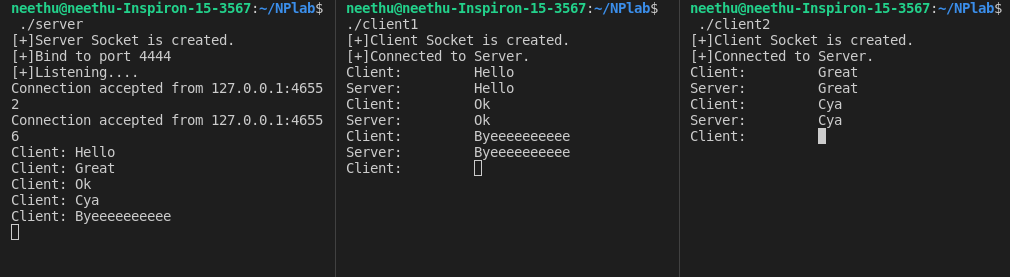
\includegraphics[scale=0.47]{img/e9.png}
\end{figure}

\subsection{Result}
Implemented the program for a multi user chat server using TCP as transport layer protocol using C language in Ubuntu 20.04 with kernel and the above outputs were obtained.

